% Component view subsection, to be included in architecture.tex

\subsection{Component view}
This section illustrates the components of the application. Figure \ref{highcomp} offers an high-level representation of the web application's modules; to keep the scheme as clear as possible and avoid modules duplication (which can result misleading), the mobile application module has been omitted, as it connects exactly like the webapp's one. The next sections offer a greater detail on the subsystems, while the components shown here are:

\begin{itemize}[itemsep=-1mm, topsep=-1mm]
	\item Maps Adapter: component used to interface the application with the mapping service's API
	\item Data Access Module: represents the system used to query the relational database 
\end{itemize}

\begin{figure}[h]	
	\centering
	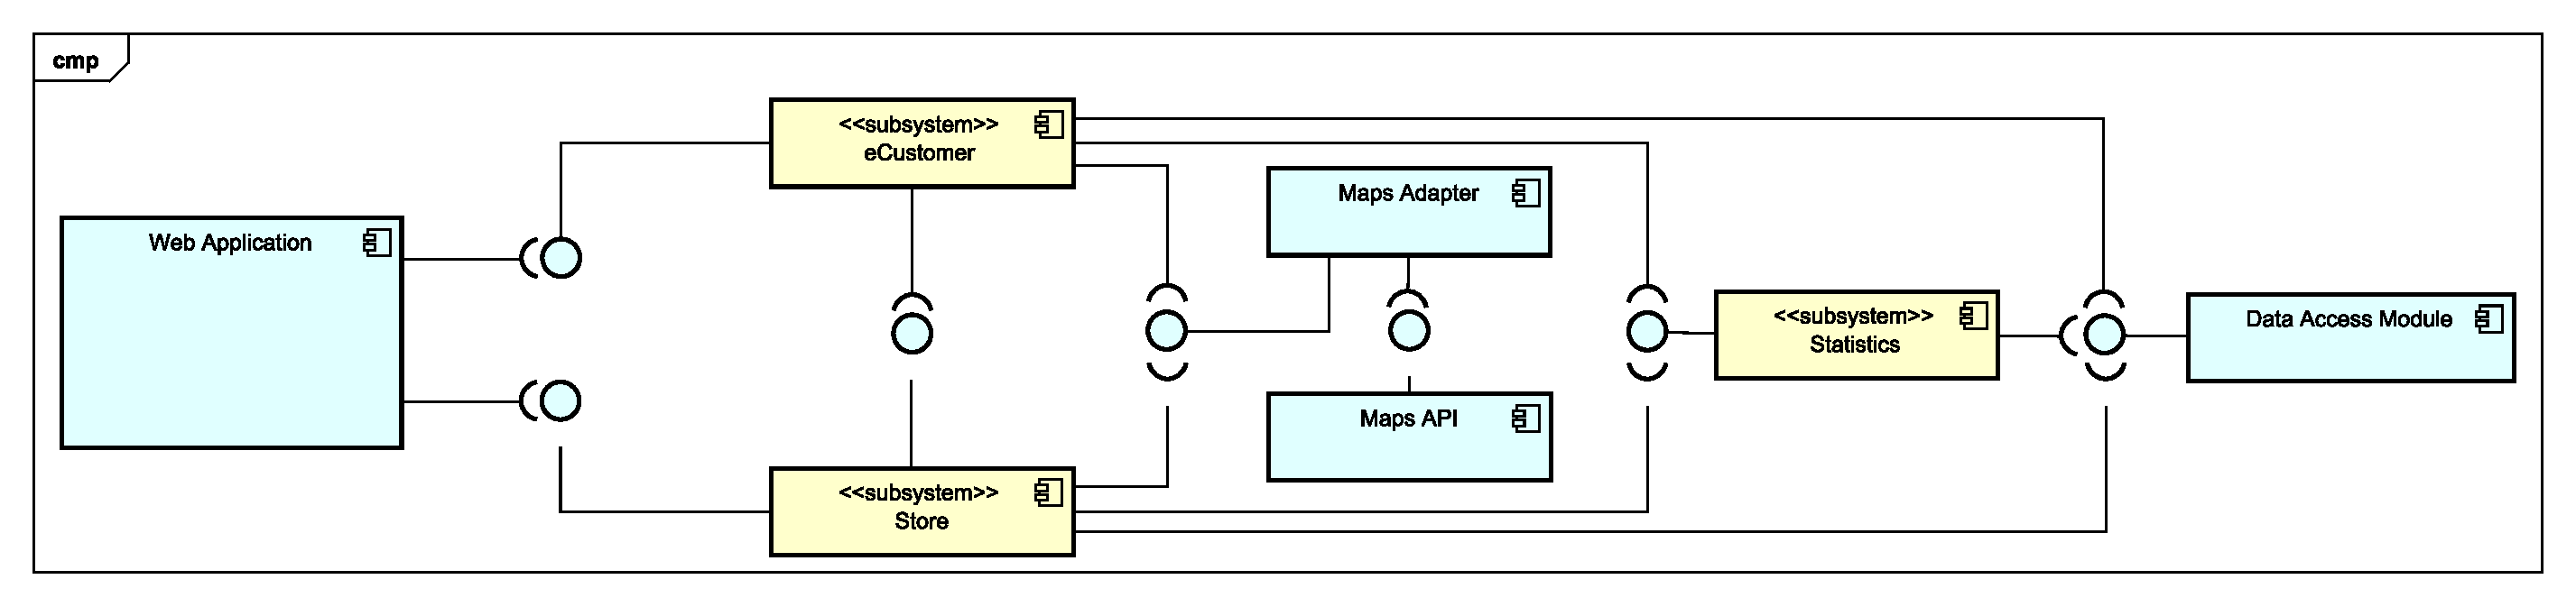
\includegraphics[width=\linewidth] {component_diagrams/component_high}
	\caption{High-level component view}
	\label{highcomp} 
\end{figure}

\subsubsection{Store subsystem}
The store subsystem modules, as shown in Figure 5, are the following:
\begin{itemize}[itemsep=-1mm, topsep=-1mm]
	\item SM Account Manager Module: allows to modify information related to the Store Manager's account
	\item Store Info Manager Module: enables the insert and update of data related to the store (capacity, delay window, items...)
	\item Access Creation Module: controls the creation of reservations and tickets (including the printing of physical ones)
	\item Queue Manager Module: manages a queue of tickets, allowing all operations such as enqueue and dequeue
	\item Visit Manager Module: is responsible for creating visits, scheduling entrances, handle delays, scan codes and manage the customers inside 
\end{itemize}\vspace{.5\baselineskip} 
The connections from components to the Account Manager to check if the Store Manager is logged in are omitted to avoid cluttering, as many modules need to check if the user can access their functions.

\subsubsection{e-Customer subsystem}
The components that realize the e-Customer subsystem are shown in Figure \ref{ecc}. They are:
\begin{itemize}[itemsep=-1mm, topsep=-1mm]
	\item eC Account Manager Module: allows the modification of the e-Customer's profile
	\item Store Recommender Module: manages the retrieval and proposal of stores to the e-Customer; considers location, travel time and store state to create its lists
	\item Access Request Module: is the module responsible for requesting the creation of tickets and reservations and handles the user interaction
	\item Requests Manager Module: controls the visualization and deletion of active tickets and reservations
	\item Notification Module: sends all notifications to the e-Customer when requested by other modules
	\item Subscription Module: handles the user's requests for slot notifications 
\end{itemize}\vspace{.5\baselineskip} 
Internal connections to the Account Manager used to check if the e-Customer is logged in are omitted.

\begin{figure}[p]	
	\centering
	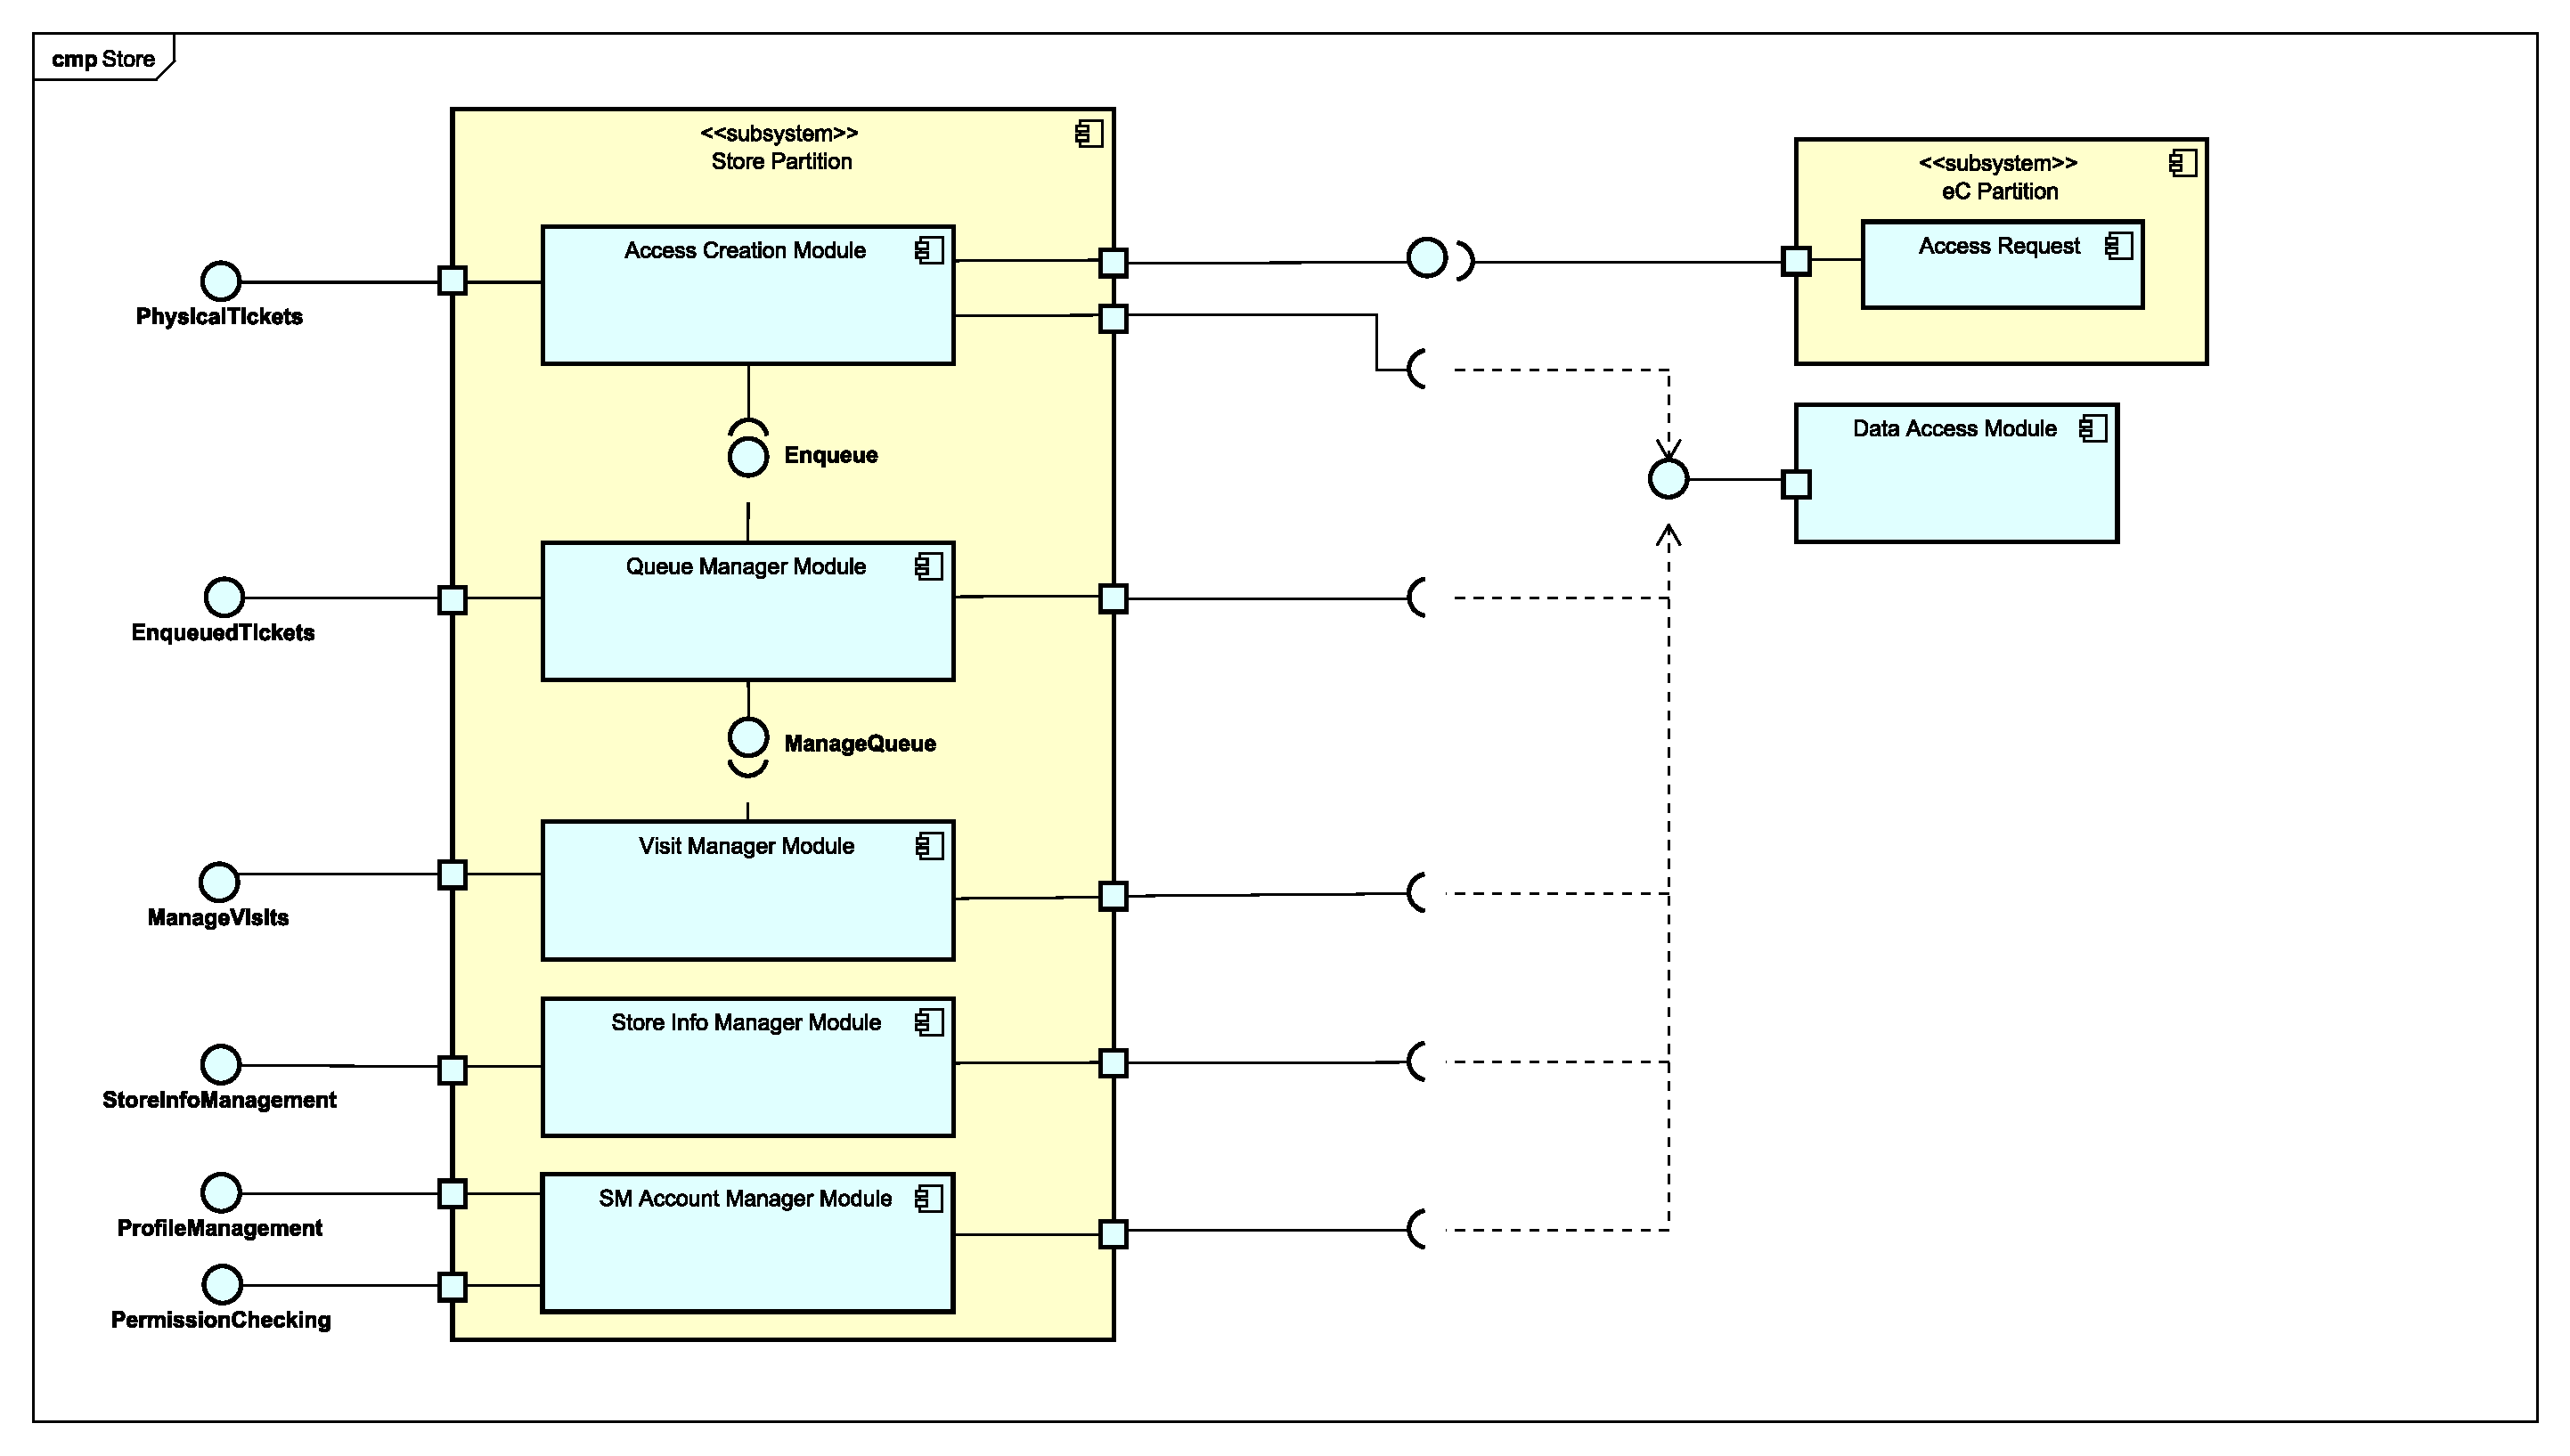
\includegraphics[width=\linewidth] {component_diagrams/component_store}
	\caption{Component view of the Store Manager subsystem}
	\label{smc} 
	
	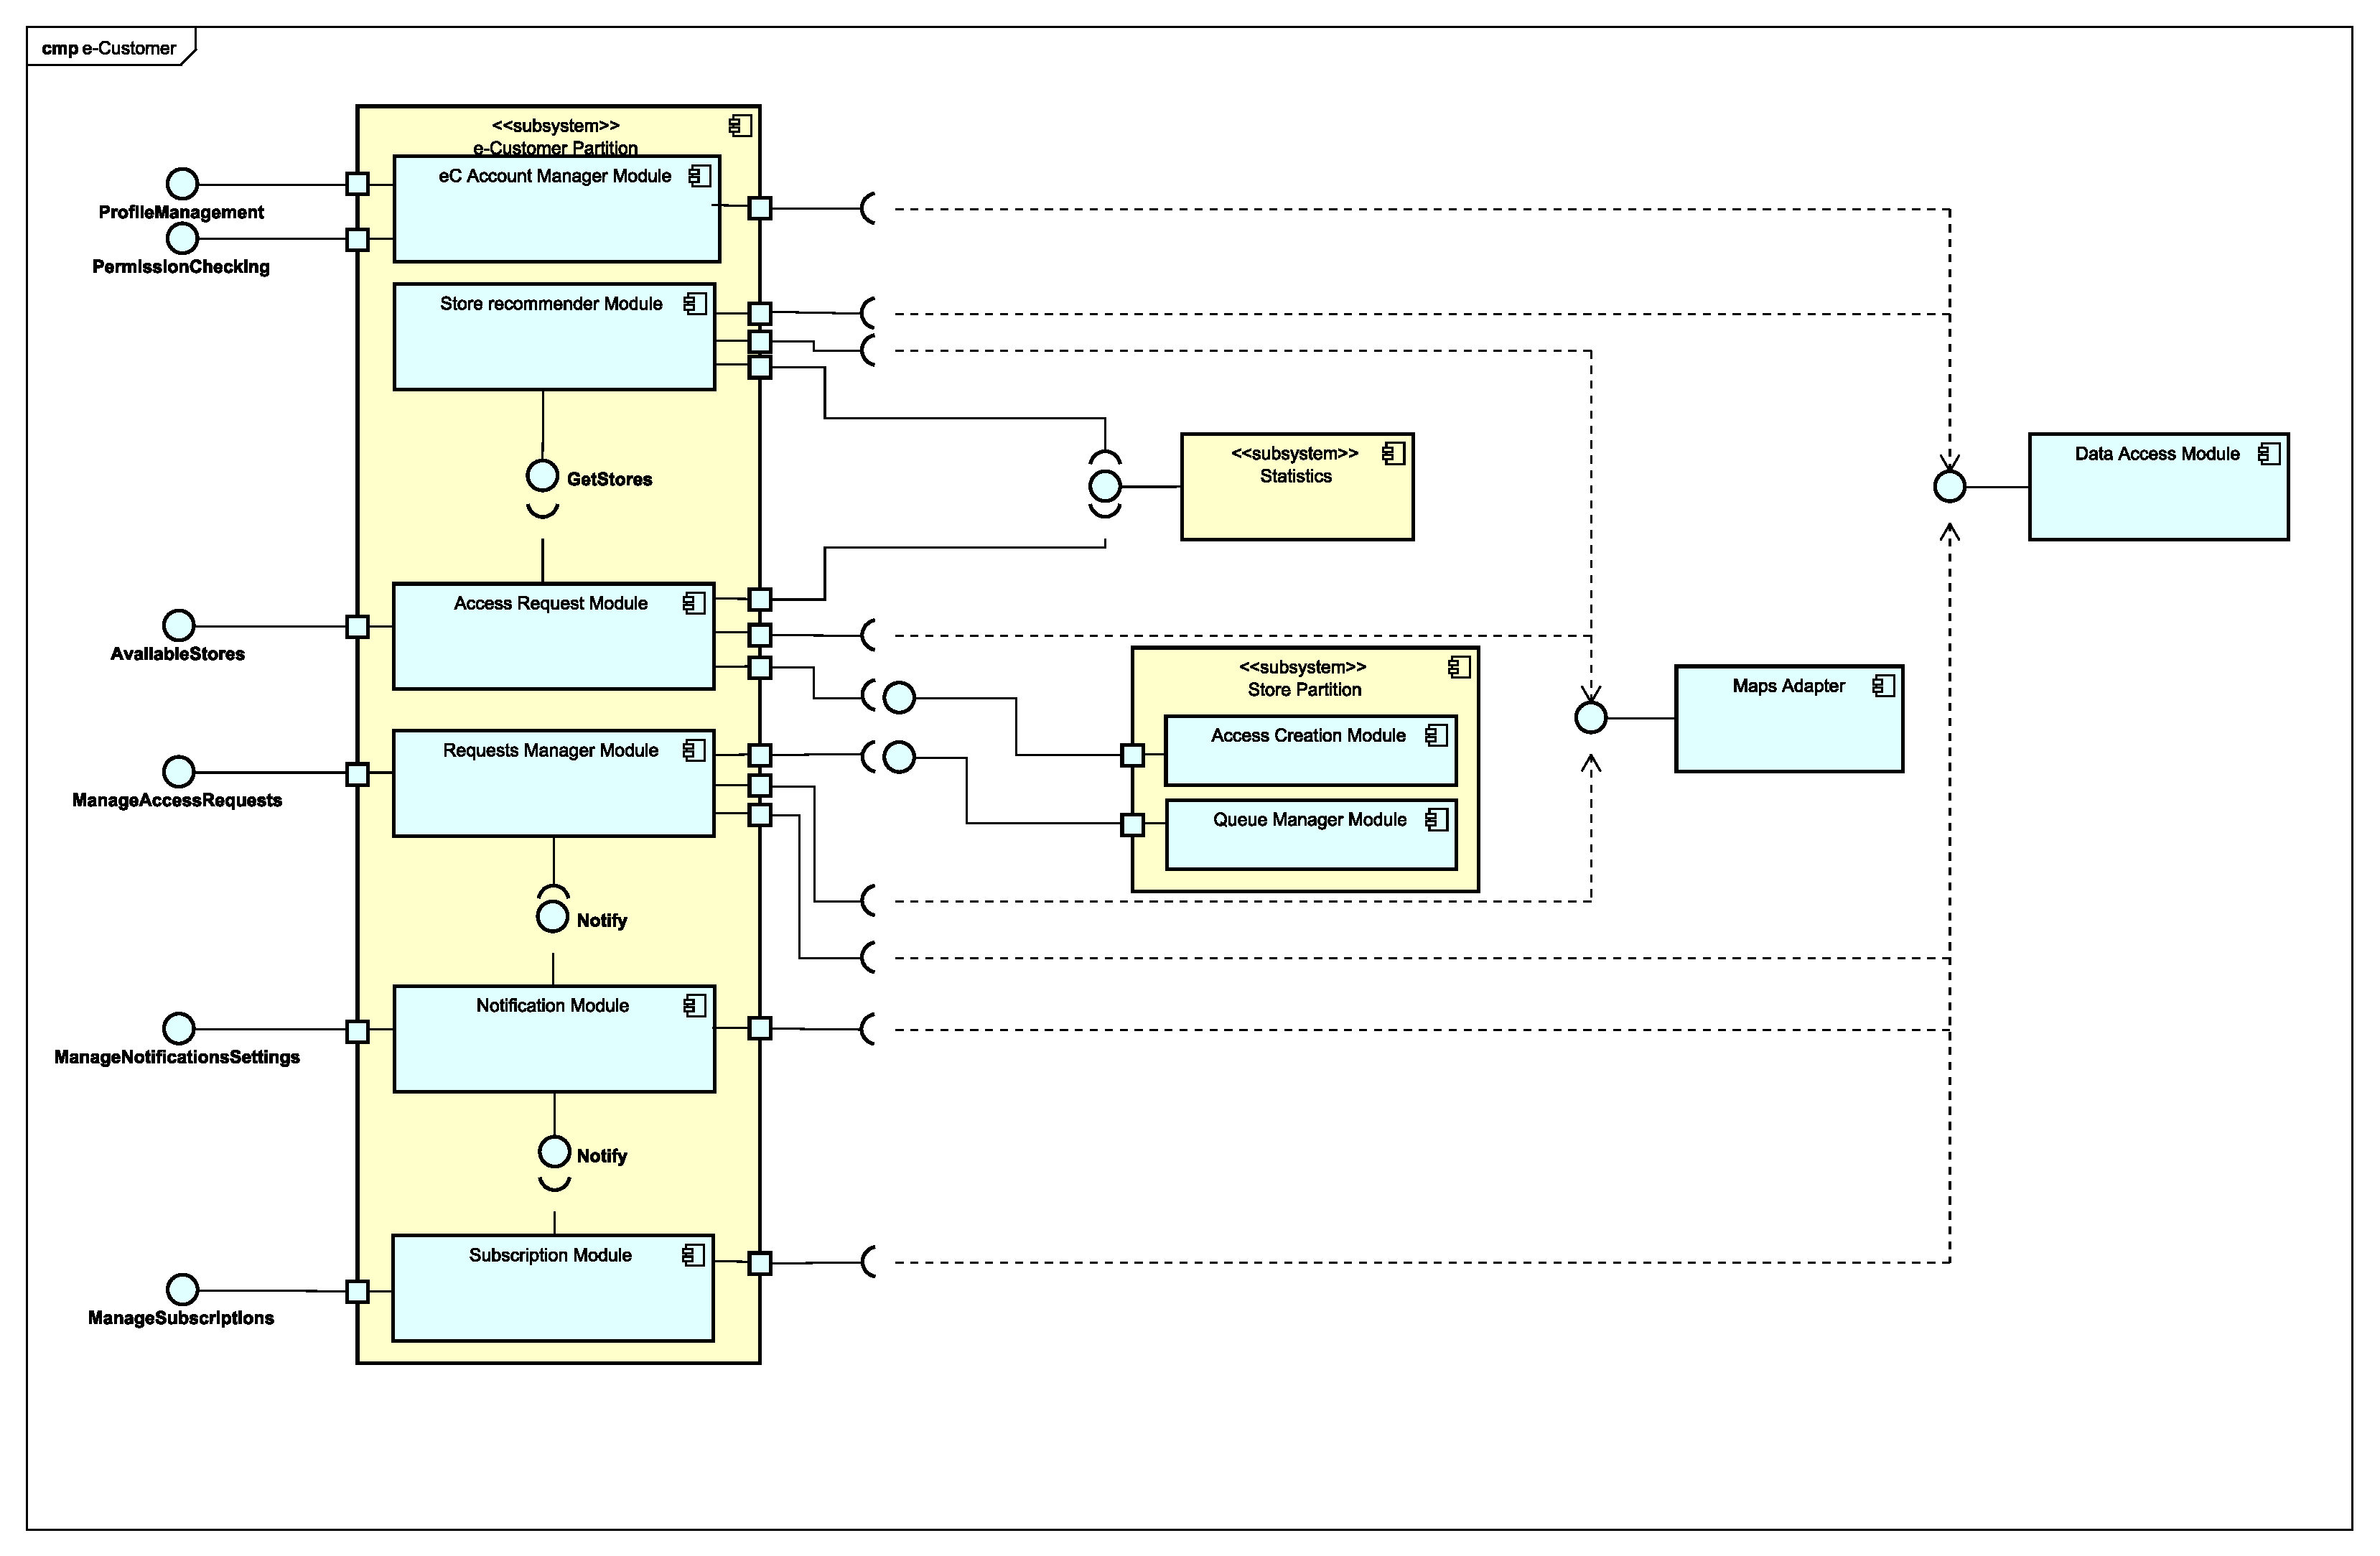
\includegraphics[width=\linewidth] {component_diagrams/component_eC}
	\caption{Component view of the e-Customer subsystem}
	\label{ecc} 
\end{figure}

\subsubsection{Statistics subsystem}
The Statistics subsystem is shown in Figure \ref{stats}. It is composed of:
\begin{itemize}[itemsep=-1mm, topsep=-1mm]
	\item Customer statistics: is responsible for elaborating data such as visit time or preferred store
	\item Store statistics: computes and aggregates data like average time of visit or mean time of queue
\end{itemize}

\begin{figure}[h]	
	\centering
	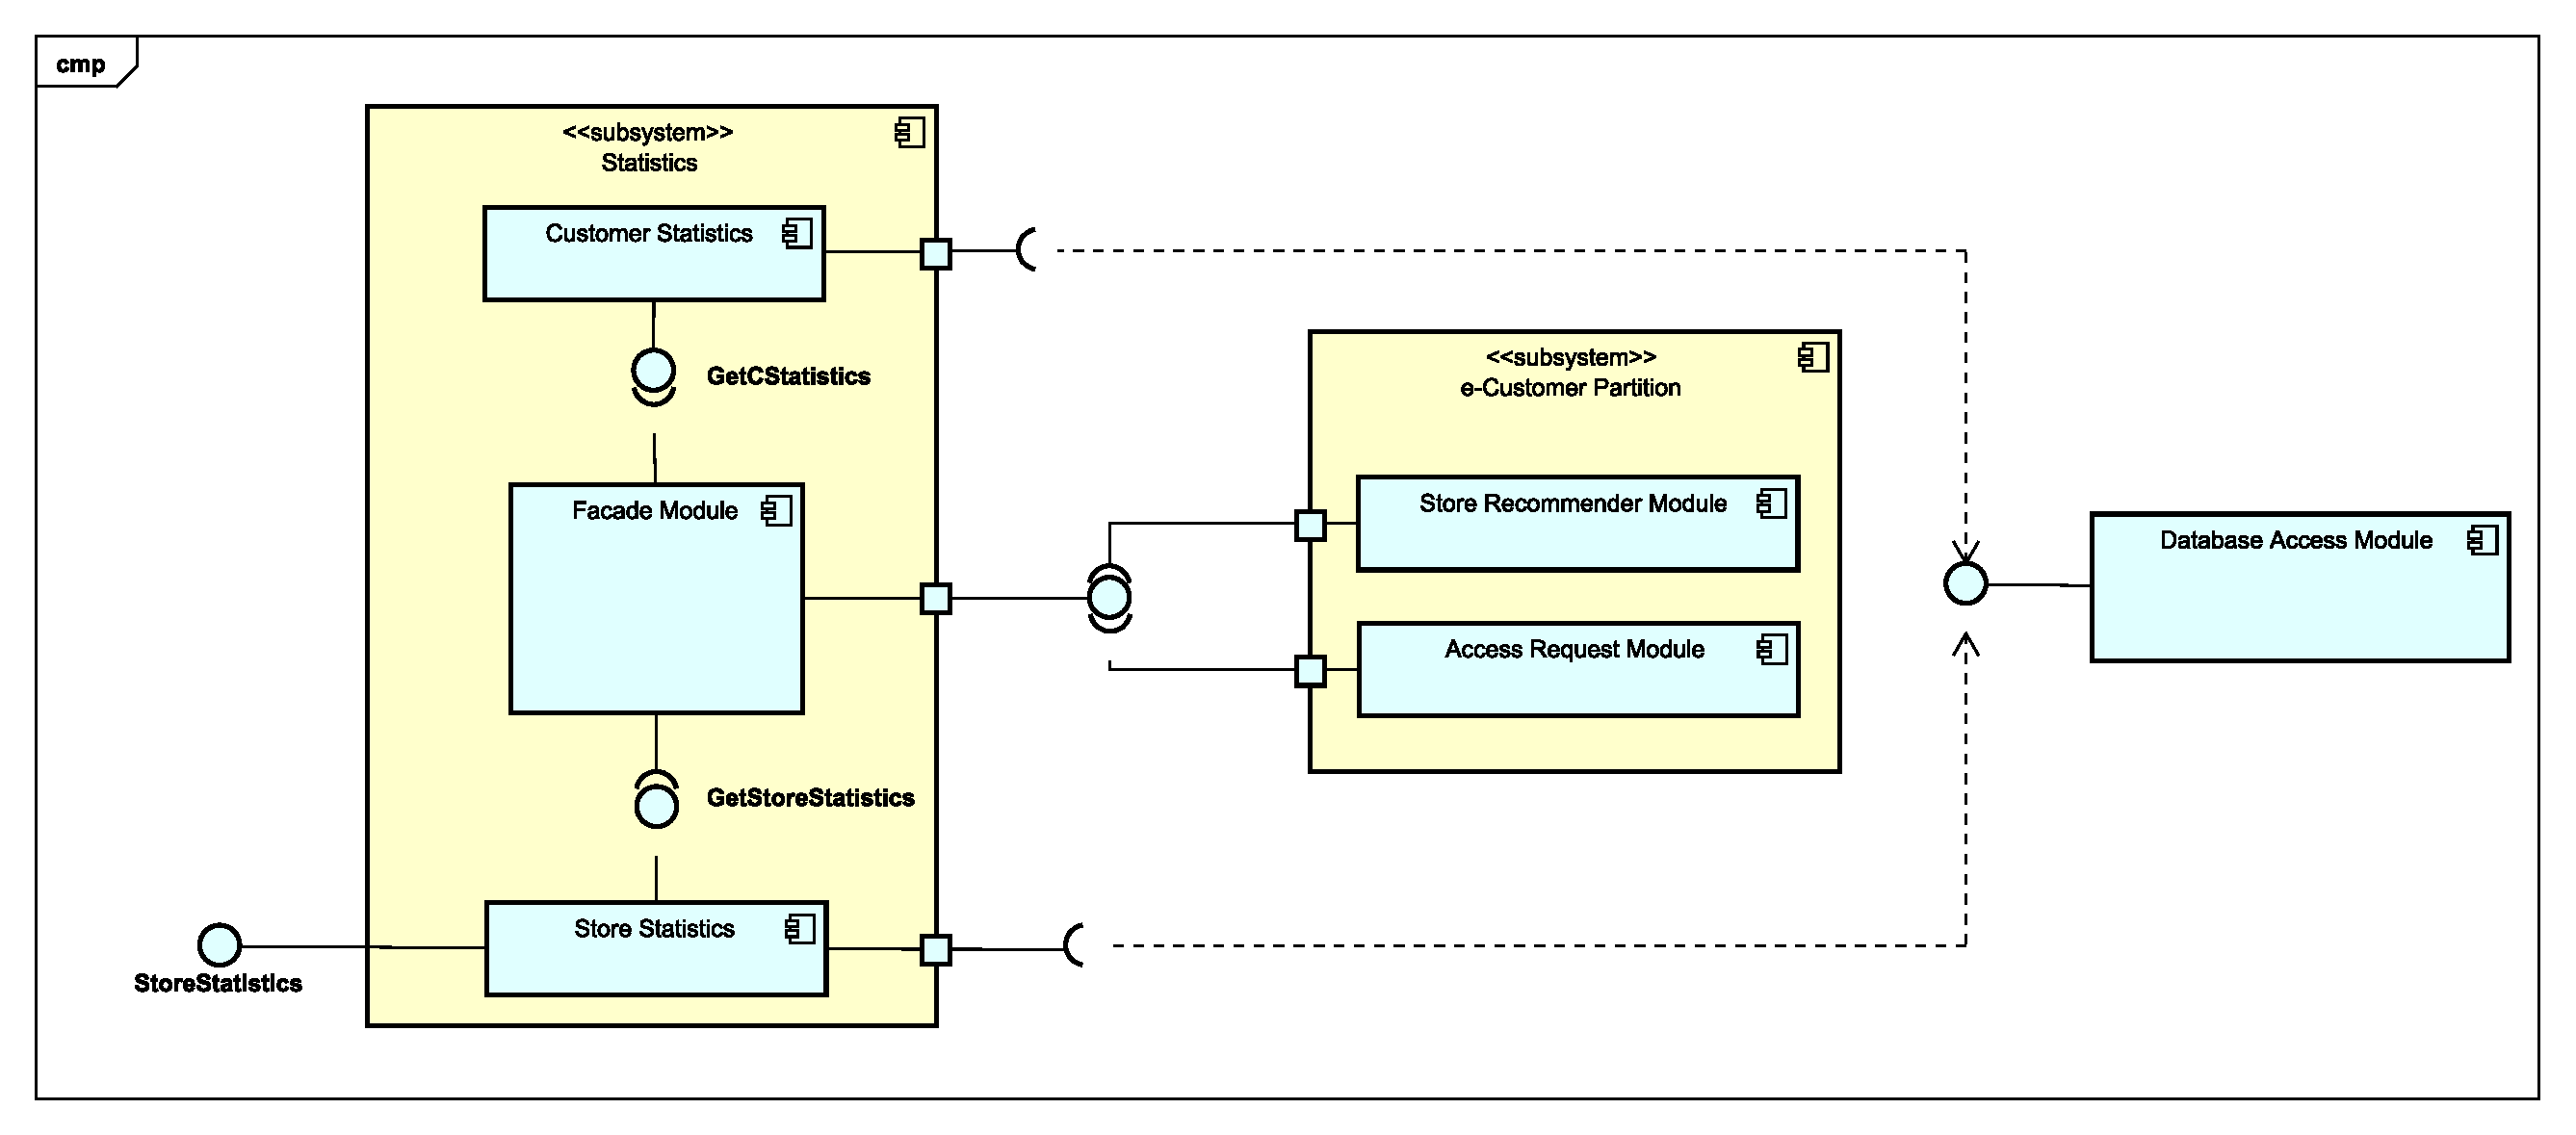
\includegraphics[width=\linewidth] {component_diagrams/statistics}
	\caption{Component view of the Statistic subsystem}
	\label{stats} 
\end{figure}
